% ============================================================================
% Appendix for PRL_attemption.tex
% Full mathematical details omitted from the 5-page PRL main text.
% ============================================================================
\documentclass[11pt]{article}

\usepackage{amsmath,amssymb,bm,geometry,graphicx,float,xcolor}
\geometry{margin=1in}

\title{Supplemental Material}
\author{Yuval Kochavi et al.}
\date{\today}

\begin{document}
\maketitle

\section*{Scope}
This supplement summarizes the working equations used in the model: the 1.5D Hammer--Rosen closure with a self-consistent Marshak boundary, wall-loss and ablation-driven density feedback terms, and the cylindrical radial eigenvalue and albedo formulation used for front curvature.

\section{The 1.5D Model}
\subsection{1D Core Equations and Marshak Closure}
We use the Hammer--Rosen (HR) 1D diffusion framework with his assumption of power-law closure~\cite{Hammer2003}. The material energy density is
\begin{equation}
\kappa^{-1}=gT^{\alpha}\rho^{-\lambda},
\qquad
e=fT^{\beta}\rho^{-\mu},
\end{equation}
and the front relation
\begin{equation}
x_F^2(t)=\frac{2+\varepsilon}{1-\varepsilon}C\,H^{-\varepsilon}(t)\int_0^t H(t')\,dt',
\qquad H(t)=T_s^{4+\alpha}(t),
\label{eq:xF_HR_appendix}
\end{equation}
with $\varepsilon=\beta/(4+\alpha)$ and $C=\frac{16g\sigma_{\mathrm{SB}}}{3f(4+\alpha)}\rho^{2-\mu-\lambda}$.

To evolve the Marshak boundary self-consistently (instead of prescribing $T_s$), we solve the following three coupled relations at each time step ~\cite{Cohen2018,Cohen2020Key}:
\begin{equation}
E(t)=f\rho^{1-\mu}(1-\varepsilon)x_F(t)H^{\varepsilon}(t),
\label{eq:E_HR_appendix}
\end{equation}
\begin{equation}
\dot E(t)=F(0,t),
\label{eq:dEdt_flux_appendix}
\end{equation}
\begin{equation}
\sigma_{\mathrm{SB}}T_D^4(t)=\sigma_{\mathrm{SB}}T_s^4(t)+\frac{1}{2}F(0,t).
\label{eq:marshak_bc_appendix}
\end{equation}
Numerically, $E$ is advanced from the boundary flux, $T_s$ is recovered from the Marshak condition, and then Eq.~\eqref{eq:xF_HR_appendix} is updated for $x_F(t)$, A more detailed description of the numerical procedure is given in the appendix of Ref.~\cite{Cohen2018}.

\subsection{Wall-Energy Loss: Full Integral Form}
Let $t_0(x)$ denote the front-arrival time at axial position $x$. After the front arrives, the local wall element is exposed for $\Delta t_x=t-t_0(x)$. For wall material $m$ (Au/Cu/Be), the absorbed areal energy is described by self-similar laws~\cite{Shussman2015,Cohen2020Key}. The governing scalings differ between subsonic and supersonic regimes because, in the subsonic case, hydrodynamic effects cannot be neglected. In this work, we use the constant boundary temperature form, since the sensitivity to the exact boundary condition is small for the present parameter range, and we treat it as if the model has constant temperatue for the time step. The subsonic expressions are applied to the high- and mid-$Z$ materials considered here, namely Au and Cu.
\begin{equation}
E_{w,\mathrm{Au}}(\Delta t_x)\simeq0.59\,T_0^{3.35}\,\Delta t_x^{0.59}
\quad [\mathrm{hJ/mm^2}],
\label{eq:wall_Au_fit_appendix}
\end{equation}
\begin{equation}
E_{w,\mathrm{Cu}}(\Delta t_x)\simeq1.58\,T_0^{3.4}\,\Delta t_x^{0.61}
\quad [\mathrm{hJ/mm^2}].
\end{equation}
Some experimental data for Be sleeve, which is supersonic under our consitions, is also available, so we need it's supersonic expression. Furthermore, for comparison to the 2D simulation without hydrodynamics, we use the corresponding supersonic-form expressions for Au/Cu:
\begin{equation}
E_{w,\mathrm{Be}}(\Delta t_x)\simeq1.71\,T_0^{4.99}\,\Delta t_x^{0.5},
\end{equation}
\begin{equation}
E_{w,\mathrm{Au}}(\Delta t_x)\simeq0.175\,T_0^{3.55}\,\Delta t_x^{0.5},
\end{equation}
\begin{equation}
E_{w,\mathrm{Cu}}(\Delta t_x)\simeq0.4\,T_0^{3.78}\,\Delta t_x^{0.5}.
\end{equation}

The total wall-loss energy is then
\begin{equation}
E_W(t)=2\pi R\int_0^{x_F(t)}\int_{0}^{t}H(t'-t_0(x))\,\dot E_{mat}\!\left(t'\right)dxdt'.
\label{eq:EW_total_appendix}
\end{equation}
Whre H is the Heaviside function, and $\dot E_{mat}$ is the appropriate wall material energy loss function. When the tube effectively has no wall, the leakage can be approximated as emission to vacuum~\cite{Cohen2020Key}. In this case, $\dot E_{mat}$ is efficiently replaced by $\sigma_{\mathrm{SB}}T(x,t)^4$. 

\subsection{Wall Ablation and Density Feedback}
Again, we use self-similar subsonic scaling laws for the high- and mid-$Z$ sleeves (Au/Cu)~\cite{Shussman2015,Cohen2020Key}. For Au and Cu, the fitted expressions used in the model are
\begin{equation}
u_{w,\mathrm{Au}}\simeq510.1\,\tilde u(\rho_{\mathrm{Au}})\,T_0^{0.716}\,\Delta t_x^{0.036}
\quad [\mathrm{km/s}].
\end{equation}
\begin{equation}
u_{w,\mathrm{Cu}}\simeq464\,\tilde u(\rho_{\mathrm{Cu}})\,T_0^{0.55}\,\Delta t_x^{0.0348}
\quad [\mathrm{km/s}].
\end{equation}
Here $\tilde u(\rho)$ (Fig.~\ref{fig:u_tilde}) is the density-dependent factor from the self-similar velocity profile, bounded between $\tilde u=1$ at the wall surface and $\tilde u=0$ at the heat front inside the wall material. In the strict self-similar derivation this profile is obtained for a free surface, while in the present problem the ablating sleeve is confined by finite-density foam. Following the calibration procedure used in our 2D simulations, we therefore evaluate this factor at a representative confined density scale of order $\rho \approx 4\,\rho_{\mathrm{foam}}$ which was a fitted parameter to our experiments. 

\begin{figure}[h!]
	\centering
	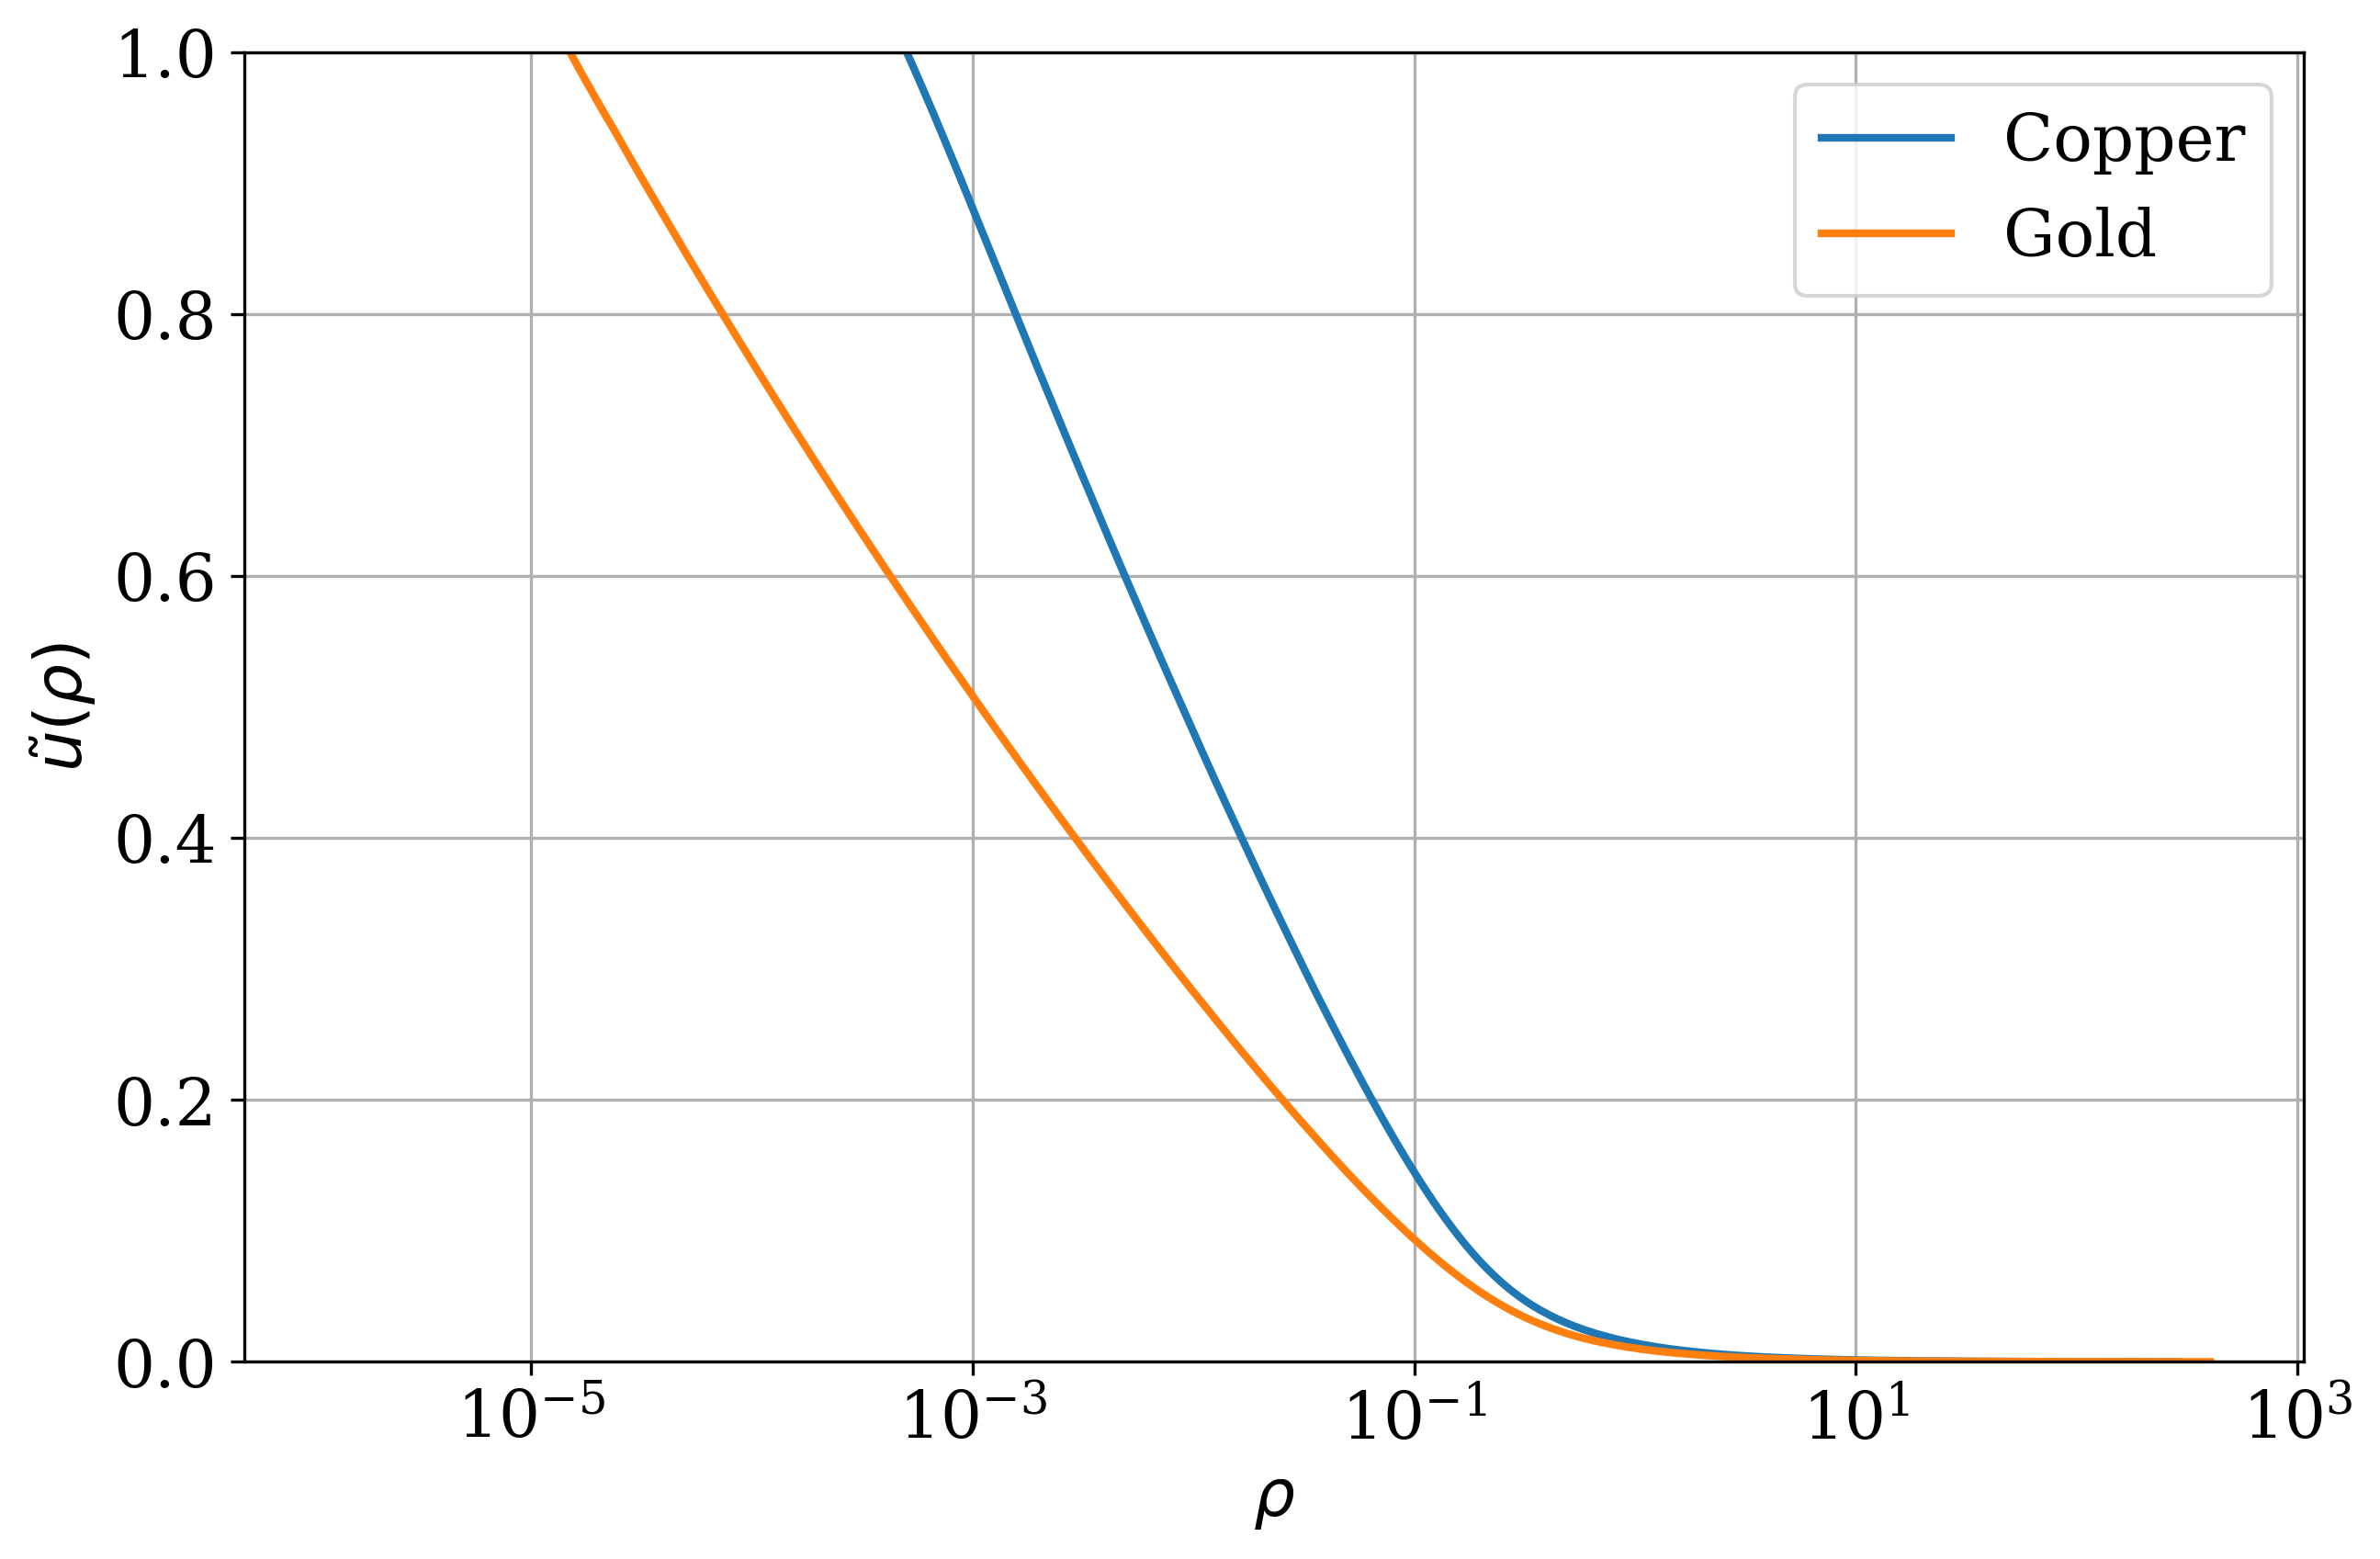
\includegraphics[width=0.5\columnwidth]{figures/u_tilda.png}
	\caption{The density-dependent factor $\tilde u(\rho)$ used in the wall-ablation velocity expressions as a function density for both Au (orange) and Cu (blue). }
	\label{fig:u_tilde}
\end{figure}

The local effective channel radius, and accordingly the heated-foam volume, then evolves as
\begin{equation}
R(x,t)=R_0-\int_{t_0(x)}^t u_w\!\left(t'-t_0(x)\right)dt', \quad V(t)=\int_0^{x_F(t)}\pi R^2(x,t)\,dx 
\label{eq:R_xt_appendix}
\end{equation}
The heated-foam volume gets smaller, and the effective mean density is updated by mass conservation. Because $C\propto\rho^{2-\mu-\lambda}$, this compression feeds back directly into the front dynamics through a time-dependent effective coefficient, which directly modifies the front evolution in Eq.~\eqref{eq:xF_HR_appendix}:
\begin{equation}
 \rho(t)=\rho_0\frac{V_0}{V(t)} \implies C(t)=\frac{16}{4+\alpha}\,\frac{g\sigma_{\mathrm{SB}}}{3ft}\int_0^t\rho^{\mu+\lambda-2}(t')\,dt'.
\label{eq:rho_update_appendix}
\end{equation}

\subsection{MFP calculation}
{\color{red}Because the temperature behind the heat wave drops spatially from $T_s(t)$ at the boundary to zero at the front depth $x_F(t)$ according to the self-similar profile $T(x,t)=T_s(t)(1-x/x_F)^{1/(4+\alpha-\beta)}$, the local mean free path $l_R(x,t)=g T^\alpha(x,t)\rho^{-\lambda-1}$ varies across the wave. Rather than evaluating the mean free path solely at the boundary temperature $T_s$, we determine the effective bulk Rosseland mean free path $\lambda_R(t)$ by integrating the optical depth across the heated region up to $0.9x_F(t)$ (excluding the steep wave tip):
\begin{equation}
    \tau(t) = \int_0^{0.9 x_F(t)} \kappa_R(x,t)\rho\,dx, \quad \lambda_R(t) = \frac{0.9\,x_F(t)}{\tau(t)}.
\end{equation}
This spatially averaged $\lambda_R(t)$ is the mean free path used in $\lambda_{\mathrm{eff}}(t)$ and throughout the model calculations.}



\section{Radial Eigenvalue Problem and Albedo Coupling}
We consider radiative heat transport in an optically thick cylindrical tube with axial coordinate $z$ and radial coordinate $r$. Under axisymmetry, LTE, constant opacity and in the steady diffusion region behind the front (neglecting the time derivative of the material energy density), the radiation field $U(z,r,t)\equiv T^4(z,r,t)$ satisfies~\cite{Hurricane2006,Courtois2022}
\begin{equation}
\frac{\partial^2 U}{\partial z^2}
+
\frac{1}{r}\frac{\partial}{\partial r}\left(r\frac{\partial U}{\partial r}\right)=0.
\label{eq:laplace_appendix}
\end{equation}
Separating variables, $U(z,r)=Z(z)R(r)$, gives a radial Bessel problem. Regularity at the axis ($r=0$) removes the singular branch, so the physical radial mode is~\cite{Hurricane2006}
\begin{equation}
R(r)=J_0(\kappa r).
\label{eq:radial_mode_appendix}
\end{equation}
To introduce albedo explicitly, let $F_{\mathrm{in}}$ be the incident radiative flux at the wall and $F_{\mathrm{out}}=\alpha F_{\mathrm{in}}$ the reflected part. The net flux absorbed by the wall is therefore $F_{\mathrm{wall}}=F_{\mathrm{in}}-F_{\mathrm{out}}=(1-\alpha)F_{\mathrm{in}}=(1-\alpha)\sigma_{\mathrm{SB}}T^4$. On the other hand, diffusion (Fick's law) gives $F_{\mathrm{wall}}=\mathbf{F}\cdot\hat{r}=-\frac{4}{3\kappa_{\mathrm{opacity}}\rho}\,\frac{\partial(\sigma_{\mathrm{SB}}T^4)}{\partial r}$. Equating the two forms gives the wall-gradient relation, which is our boundary contidion at $r=R$, with $(\alpha-1)<0$ for $\alpha<1$, i.e. the temperature decreases toward the wall~\cite{Hurricane2006,Courtois2022}:
\begin{equation}
\left.\frac{\partial U}{\partial r}\right|_{r=R}
=
\frac{3}{4}\rho\kappa_{\mathrm{opacity}}(\alpha-1)\,U(R).
\label{eq:robin_appendix}
\end{equation}
Substituting $R(r)=J_0(\kappa r)$ and using $\frac{d}{dr}J_0(\kappa r)=-\kappa J_1(\kappa r)$ leads to the eigenvalue equation~\cite{Hurricane2006,Courtois2022}
\begin{equation}
\kappa R\,J_1(\kappa R)=\varepsilon\,J_0(\kappa R),
\qquad
\varepsilon\equiv\frac{3}{4}(1-\alpha)\tau,
\qquad
\tau\equiv\rho\kappa_{\mathrm{opacity}}R,
\label{eq:eigenvalue_appendix}
\end{equation}
which determines the discrete spectrum $\{\kappa_n\}$. The physically relevant curvature scale is the lowest positive root, $\kappa_0$. In the weak-loss (high-albedo) limit, $\varepsilon\ll1$, the leading-order expansion of $J_0$ and $J_1$ gives
\begin{equation}
\kappa_0R\approx\sqrt{2\varepsilon},
\qquad
\kappa_0\approx\frac{\sqrt{2\varepsilon}}{R}.
\label{eq:kappa0_small_loss_appendix}
\end{equation}
This expression is accurate when wall absorption is small. For lower albedo (larger losses), $\kappa_0$ is obtained by numerical solution of Eq.~\eqref{eq:eigenvalue_appendix}, which is the procedure used in the model.

We now derive an expression for the time-dependent albedo. The incoming flux toward the wall is $\sigma_{\mathrm{SB}}T_0^4$, where $T_0$ is the effective temperature of the incoming flux from the foam region. The outgoing flux is $\sigma_{\mathrm{SB}}T_{\mathrm{obs}}^4$, \textcolor{red}{where $T_{\mathrm{obs}}$ is the brightness temperature (alternatively, the temperature at about $2/3$ mfp from re-emission, observed re-emission temperature)}. Energy conservation gives
$\sigma_{\mathrm{SB}}T_0^4 = \sigma_{\mathrm{SB}}T_{\mathrm{obs}}^4 + F(0,t)$,
where $F(0,t)$ is the flux absorbed by the wall and therefore satisfies $F(0,t)=\partial E_W/\partial t$. The detector measures the re-emitted flux, equal to the sum of wall emission and half of the absorbed flux. The quantities $T_{\mathrm{obs}}$ and $T_0$ are not directly known, but the interface temperature is known from the Henyey-like profile ~\cite{Hammer2003} at the foam surface ($x=0$), denote it by $T_{\mathrm{int}}$. Using the Marshak boundary condition at the interface, we have:

\begin{equation}
\sigma_{SB} T_{0}^4 = \sigma_{SB} T_{int}^4 + \frac{F(0,t)}{2}
\end{equation}

Therefore, we can write:
\begin{equation}
\sigma_{\mathrm{SB}}T_{\mathrm{obs}}^4 = \sigma_{SB} T_{int}^4 - \frac{F(0,t)}{2}
\end{equation}

And now we can use the albedo definition to calculate it:

\begin{equation}
\alpha (t)
=
\frac{F_{\text{out}}}{F_{\text{in}}}
=
\frac{\sigma_{\mathrm{SB}}T_{\mathrm{obs}}^4}{\sigma_{\mathrm{SB}}T_0^4}
=
\frac{\sigma_{\mathrm{SB}}T_0^4 - \frac{\dot{E}_w}{2}}{\sigma_{\mathrm{SB}}T_0^4 + \frac{\dot{E}_w}{2}}
\end{equation}
\section{Simulation details}
The simulation introduced in the letter is a 2D diffusion simulation without hydrodynamics, using cylindral geometry. The equations discritization is done through finite diffrencing on the coupled equations, which are the boltzman equation under moments development and using the diffusion approximation (Eq.~\eqref{eq:E_continuous_conservative}), and the material energy equation (Eq.~\eqref{eq:U_continuous}). The equations are as follows:
\begin{equation}
\frac{\partial E}{\partial t}
=
\frac{1}{r}\frac{\partial}{\partial r}\left(rD\frac{\partial E}{\partial r}\right) + \frac{\partial}{\partial z}\left(D\frac{\partial E}{\partial z}\right)
-
\chi c\sigma(E - U_R).
\label{eq:E_continuous_conservative}
\end{equation}

\begin{equation}
\frac{1}{\gamma}\,\frac{\partial U_R}{\partial t}
=
\chi c\sigma(E - U_R),
\label{eq:U_continuous}
\end{equation}
Here $E=aT_R^4$ is the radiation energy density (with $a$ the radiation constant), $T_R$ is the radiation temperature, and $T_m$ is the material temperature. The material internal-energy density is
\begin{equation}
U_m\equiv \rho e = fT_m^{\beta}\rho^{1-\mu},
\end{equation}
using the same power-law closure adopted in the model. The transport mean free path is written as
\begin{equation}
\frac{1}{\sigma}=\frac{1}{\kappa\rho}=gT_m^{\alpha}\rho^{-(\lambda+1)},
\end{equation}
and we define
\begin{equation}
U_R\equiv aT_m^4,
\qquad
\gamma\equiv\frac{\partial U_R}{\partial U_m},
\qquad
D\equiv\frac{c}{3\sigma},
\end{equation}
where $D$ is the diffusion coefficient and $c$ is the speed of light.

The simulation is performed on a 2D $(r,z)$ grid: uniform spacing in $z$, and a piecewise radial mesh that is uniform in the foam ($r<R_{\mathrm{tube}}$) and geometrically stretched in the coating region ($R_{\mathrm{tube}}<r<R_{\mathrm{tube}}+\omega_{\mathrm{coat}}$). This allows accurate resolution of the large velocity contrast between foam and coating heating.

Boundary conditions are: symmetry at the axis ($r=0$); no active outer-wall condition at $r=R_{\mathrm{tube}}+\omega_{\mathrm{coat}}$ because the front does not reach that boundary over the simulated time; and no active downstream condition at $z=L$ for the same reason. The simulation outputs are $E(r,z,t)$ and $U_m(r,z,t)$ at each time step.

\section{Material and Experimental Database}
This section summarizes the experimental set used for comparison and the material-fit coefficients used throughout the model. Table~\ref{tab:supported_experiments} lists the relevant foam compositions, density and temperature ranges, and reference groups. Table~\ref{tab:material_fits} provides the corresponding power-law parameters $\left(g,f,\alpha,\beta,\lambda,\mu\right)$ used in both model and simulation. Together, these tables define the input database used to generate the front-evolution and curvature results reported in the manuscript.

\begin{table}[!htbp]
\centering
\small
\renewcommand{\arraystretch}{1.1}
\begin{tabular}{lcccc}
\hline
The experiment & foam type & density (mg/cc) & temperature (eV) & Ref.\\
\hline
Back $et\ al.$ & SiO$_2$, Ta$_2$O$_5$ & 10--50 & 85--190 & ~\cite{Back2000PRL,Back2000POP}\\
Courtois $et\ al.$ & SiO$_2$ & 18.9, 29 & 100--180 & ~\cite{Courtois2024}\\
\hline
\end{tabular}
\caption{Experimental platforms and conditions summarized from the supported-material references used in the manuscript.}
\label{tab:supported_experiments}
\end{table}

\begin{table}[!htbp]
\centering
\small
\renewcommand{\arraystretch}{1.1}
\begin{tabular}{lccccccc}
\hline
Experiment name & Foam & $g$ (g/cm$^2$) & $f$ (MJ) & $\alpha$ & $\beta$ & $\lambda$ & $\mu$ \\
\hline
Back, Courtois & SiO$_2$ & 1/9175 & 8.77 & 3.53 & 1.1 & 0.75 & 0.09 \\
Back & Ta$_2$O$_5$ & 1/8433.3 & 4.78 & 1.78 & 1.37 & 0.24 & 0.12 \\
Back low energy & SiO$_2$ & 1/9652 & 8.4 & 2.0 & 1.23 & 0.61 & 0.1 \\
 & Au & 1/7200 & 3.4 & 1.5 & 1.6 & 0.2 & 0.14 \\
 & Be & 1/402.8 & 8.81 & 4.89 & 1.09 & 0.67 & 0.07 \\
 & Cu & 1/2237 & 5.7 & 2.21 & 1.35 & 0.29 & 0.14 \\
\hline
\end{tabular}
\caption{Material fit parameters used in the model for the supported experimental platforms and coating materials.}
\label{tab:material_fits}
\end{table}


\begin{thebibliography}{99}

\bibitem{Hammer2003}
J.~H.~Hammer and M.~D.~Rosen,
\textit{A consistent approach to solving the radiation diffusion equation},
Phys.\ Plasmas \textbf{10}, 1829 (2003).

\bibitem{Shussman2015}
T.~Shussman and S.~I.~Heizler,
\textit{Full self-similar solutions of the subsonic radiative heat equations},
Phys.\ Plasmas \textbf{22}, 082109 (2015).

\bibitem{Pomraning1979}
G.~C.~Pomraning,
\textit{The Equations of Radiation Hydrodynamics}
(Pergamon, Oxford, 1973).

\bibitem{Fleck1971}
J.~A.~Fleck, Jr., and J.~D.~Cummings, Jr.,
\textit{An implicit Monte Carlo scheme for calculating time and frequency dependent nonlinear radiation transport},
J.~Comput.~Phys.~\textbf{8}, 313 (1971).

\bibitem{Su1996}
B.~Su and G.~L.~Olson,
\textit{Benchmark results for the non-equilibrium Marshak diffusion problem},
J.~Quant.~Spectrosc.~Radiat.~Transfer~\textbf{56}, 337 (1996).

\bibitem{Back2000PRL}
C.~A.~Back, J.~D.~Bauer, J.~H.~Hammer \textit{et al.},
\textit{Diffusive, supersonic x-ray transport in radiatively heated foam cylinders},
Phys.\ Rev.\ Lett.\ \textbf{84}, 274 (2000).

\bibitem{Back2000POP}
C.~A.~Back, J.~D.~Bauer, O.~L.~Landen \textit{et al.},
\textit{Detailed measurements of a diffusive supersonic wave in a radiatively heated foam},
Phys.\ Plasmas \textbf{7}, 2126 (2000).

\bibitem{Cohen2018}
A.~P.~Cohen and S.~I.~Heizler,
J.\ Comput.\ Theor.\ Transp.\ \textbf{47}, 378 (2018).

\bibitem{Cohen2020Key}
A.~P.~Cohen, G.~Malamud, and S.~I.~Heizler,
\textit{Key to understanding supersonic radiative Marshak waves using simple models and advanced simulations},
Phys.\ Rev.\ Research \textbf{2}, 023007 (2020).

\bibitem{Hurricane2006}
O.~A.~Hurricane and J.~H.~Hammer,
\textit{Bent Marshak waves},
Phys.\ Plasmas \textbf{13}, 113303 (2006).

\bibitem{Courtois2022}
C.~Courtois, R.~Gr\"oger, P.~Loiseau \textit{et al.},
\textit{Models for the propagation of radiation heat fronts in cylindrical tubes},
Phys.\ Plasmas \textbf{29}, 022704 (2022).

\bibitem{Courtois2024}
C.~Courtois, R.~Gr\"oger, P.~Loiseau \textit{et al.},
\textit{Experimental measurements of supersonic radiation heat wave curvature in cylindrical tubes},
Phys.\ Plasmas \textbf{31}, 012707 (2024).

\end{thebibliography}
\end{document}

